\section{Curva CTR del optoacoplador 4N25}
 
\subsection{Circuito de medición}
 
Para medir la curva del CTR se utilizó el circuito de la figura~\ref{fig:circuito_ctr}.
El LED interno se polarizó con una fuente variable $V_{cc}$ en serie con dos resistencias:
$R_s = \SI{50}{\ohm}$ (resistencia interna de la fuente) y $R = \SI{28}{\ohm}$ adicional,
dando una resistencia total de $R_{total} = \SI{78}{\ohm}$, utilizada para limitar la corriente.


La salida del fototransistor se cargó con $R_C = \SI{980}{\ohm}$ a $V_{ceo} = \SI{20}{V}$.
Las corriente $I_F$ e $I_C$ se midieron calculando la caída de tensión en las resistencias y conociendo sus valores
se implementó la ley de ohm. Luego el CTR se calculó de la sigueinte forma:
\begin{equation}
    \mathrm{CTR} = \frac{I_C}{I_F}.
\end{equation}
 
% ---- Circuito con circuitikz ----
\begin{figure}[H]
    \centering
    \begin{circuitikz}[american, scale=0.9]
        
        % --- Lado entrada (LED) ---
        \draw (0,4) to[V, l=$V_{cc}$] (0,0)
                   (0,4) to[R, l=$R_s{=}\SI{50}{\ohm}$] (2.5,4)
                    to[R, l=$R{=}\SI{28}{\ohm}$] (5,4)
                    to[ammeter, l=$A_{I_F}$] (5,2)
                    to[leD, l=LED] (5,0) -- (0,0);

        % --- Lado salida (fototransistor) ---
        \draw (10,2) node[npn, anchor=C](Q){};
        \draw (Q.E) -- (10,0) node[ground]{};
        \draw (Q.B) node[left, xshift=-0.2cm]{Base (nc)}; % Agregado un pequeño shift para asegurar distancia

        % Vceo y Rc en serie hacia el colector (alineado a X=9.5)
        \draw (10,4) node[above]{$+V_{ceo}{=}\SI{20}{V}$}
                    to[R, l_=$R_C{=}\SI{980}{\ohm}$] (Q.C);

        % Voltímetro en paralelo a Rc 
        \draw (10,4) -- (11.5,4)
              to[voltmeter, l=$V_{R_C}$] (11.5,2) -- (10,2);

    \end{circuitikz}
    \caption{Circuito para medición de CTR (sin $R_{BE}$)}
    \label{fig:circuito_ctr}
\end{figure}
 
\subsection{Curva CTR: comparación con el fabricante}
 
La hoja de datos de Vishay presenta el CTR \emph{normalizado} (NCTR) referenciado a las
condiciones $V_{CE}=\SI{10}{V}$, $I_F=\SI{10}{mA}$, $T_A=\SI{25}{\celsius}$, con un
valor típico de $\mathrm{CTR_{DC}}=50\%$ para el 4N25.  Para comparar con los datos
medidos se normalizó la curva experimental dividiendo cada valor de CTR por el valor
obtenido a $I_F\approx\SI{10}{mA}$.
 
% ---- Tabla de datos medidos (Vceo = 20 V) ----
\begin{table}[H]
    \centering
    \caption{Valores medidos con $V_{ceo}=\SI{20}{V}$, $R_C=\SI{980}{\ohm}$, $R_{total}=\SI{78}{\ohm}$. $I_F$ e $I_C$ medidos con amperímetros.}
    \label{tab:ctr_medido}
    \sisetup{round-mode=places, round-precision=3}
    \begin{tabular}{
        S[table-format=1.2]  % Vcc
        S[table-format=2.2]  % V_RC
        S[table-format=2.3]  % Ic
        S[table-format=2.4]  % If
        S[table-format=1.4]  % CTR
    }
        \toprule
        {$V_{cc}$ (V)} & {$V_{RC}$ (V)} & {$I_C$ (mA)} & {$I_F$ (mA)} & {CTR} \\
        \midrule
        1.10 & 0.27  & 0.275  & 0.3570  & 0.7703 \\
        1.20 & 1.59  & 1.622  & 2.1400  & 0.7579 \\
        1.30 & 3.60  & 3.683  & 3.5700  & 1.0317 \\
        1.40 & 6.95  & 7.090  & 6.0700  & 1.1680 \\
        1.50 & 9.53  & 9.720  & 7.8500  & 1.2382 \\
        1.61 & 13.31 & 13.580 & 10.700  & 1.2692 \\
        1.70 & 14.73 & 15.030 & 6.4100  & 2.3447 \\
        1.81 & 18.92 & 19.300 & 7.8200  & 2.4679 \\
        1.91 & 19.35 & 19.750 & 9.1025  & 2.1698 \\
        2.00 & 19.46 & 19.850 & 10.256  & 1.9354 \\
        2.14 & 19.73 & 20.130 & 12.051  & 1.6704 \\
        2.30 & 19.82 & 20.220 & 14.103  & 1.4338 \\
        2.39 & 19.93 & 20.330 & 15.256  & 1.3326 \\
        2.49 & 20.00 & 20.408 & 16.538  & 1.2340 \\
        \bottomrule
    \end{tabular}
\end{table}
 
% ---- Gráfico CTR vs IF ----
% Reemplazar los datos inline por \addplot table si se dispone del .csv
 
\begin{figure}[H]
    \centering
    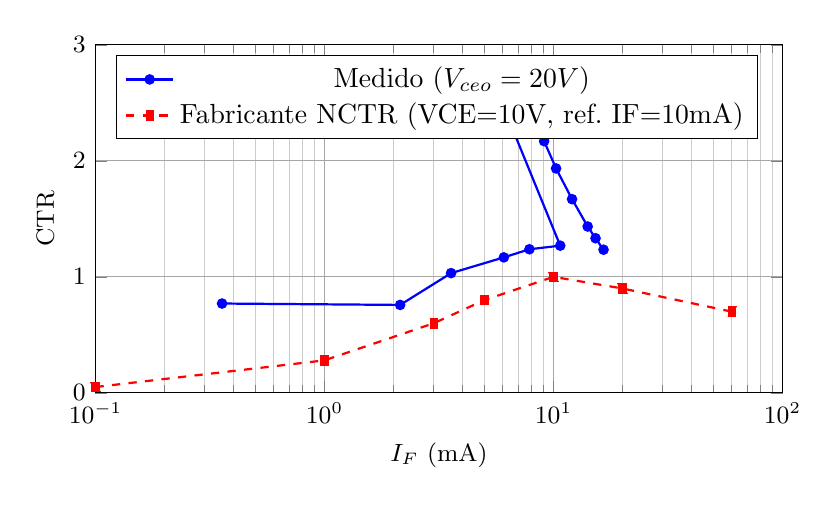
\begin{tikzpicture}
        \begin{semilogxaxis}[
            width=0.85\linewidth, height=6cm,
            xlabel={$I_F$ (mA)},
            ylabel={CTR},
            xmin=0.1, xmax=100,
            ymin=0,   ymax=3,
            legend pos=north west,
            grid=both,
            grid style={line width=0.2pt, draw=gray!40},
            major grid style={line width=0.4pt, draw=gray!70},
            tick label style={font=\small},
            label style={font=\small},
        ]
            % --- Curva medida (no saturada) ---
            \addplot[blue, thick, mark=*, mark size=1.5pt]
                coordinates {
                    (0.357,  0.770)
                    (2.14,   0.758)
                    (3.57,   1.032)
                    (6.07,   1.168)
                    (7.85,   1.238)
                    (10.7,   1.269)
                    (6.41,   2.345)
                    (7.82,   2.468)
                    (9.10,   2.170)
                    (10.26,  1.935)
                    (12.05,  1.670)
                    (14.10,  1.434)
                    (15.26,  1.333)
                    (16.54,  1.234)
                };
            \addlegendentry{Medido ($V_{ceo}=\SI{20}{V}$)}
 
            % --- Referencia fabricante: CTR_DC tipico = 50% a IF=10mA, VCE=10V
            %     Curva normalizada tipica (aproximacion lineal-log del datasheet Fig.2)
            \addplot[red, dashed, thick, mark=square*, mark size=1.5pt]
                coordinates {
                    (0.1,  0.05)
                    (1,    0.28)
                    (3,    0.60)
                    (5,    0.80)
                    (10,   1.00)
                    (20,   0.90)
                    (60,   0.70)
                };
            \addlegendentry{Fabricante NCTR (VCE=10V, ref.\ IF=10mA)}
        \end{semilogxaxis}
    \end{tikzpicture}
    \caption{CTR medido vs.\ curva normalizada del fabricante.
             La curva del fabricante (Fig.~2 del datasheet) está normalizada al valor de
             $\mathrm{CTR_{DC}}$ a $I_F=\SI{10}{mA}$, $V_{CE}=\SI{10}{V}$;
             la curva medida se normalizó al valor experimental en esa misma condición.}
    \label{fig:ctr_vs_if}
\end{figure}
 
\noindent\textbf{Análisis:}
La curva del fabricante es \emph{normalizada}, de modo que para comparar se dividió cada
punto medido por el CTR obtenido a $I_F\approx\SI{10}{mA}$.
Para corrientes bajas ($I_F < \SI{3}{mA}$) el CTR cae rápidamente, en concordancia con
el datasheet.  A corrientes medias el CTR sube y alcanza su máximo, para luego decrecer
por saturación del fototransistor.  El valor típico del fabricante es
$\mathrm{CTR_{DC}}=20$--$50\%$ a $V_{CE}=\SI{10}{V}$; a $V_{ceo}=\SI{20}{V}$ se
observa un comportamiento similar pero ligeramente desplazado, coherente con la
dependencia de VCE indicada en las características típicas.